% !TEX program = pdflatex
% !TEX options = -synctex=1 -interaction=nonstopmode -file-line-error "%DOC%"
% 固体物理第八次作业
\documentclass[UTF8,10pt,a4paper]{article}
\usepackage{ctex}
% \catcode`\。=\active
% \newcommand{。}{.}
\newcommand{\CourseName}{固体物理}
\newcommand{\CourseCode}{PHYS1502}
\newcommand{\Semester}{2019-2020学年第二学期}
\newcommand{\ProjectName}{第八次作业}
\newcommand{\DueTimeType}{截止时间}
\newcommand{\DueTime}{2020. 5. 1(周五)17:00}
\newcommand{\StudentName}{陈稼霖}
\newcommand{\StudentID}{45875852}
\usepackage[vmargin=1in,hmargin=.5in]{geometry}
\usepackage{fancyhdr}
\usepackage{lastpage}
\usepackage{calc}
\pagestyle{fancy}
\fancyhf{}
\fancyhead[L]{\CourseName}
\fancyhead[C]{\ProjectName}
\fancyhead[R]{\StudentName}
\fancyfoot[R]{\thepage\ / \pageref{LastPage}}
\setlength\headheight{12pt}
\fancypagestyle{FirstPageStyle}{
    \fancyhf{}
    \fancyhead[L]{\CourseName\\
        \CourseCode\\
        \Semester}
    \fancyhead[C]{{\Huge\bfseries\ProjectName}\\
        \DueTimeType\ : \DueTime}
    \fancyhead[R]{姓名 : \makebox[\widthof{\StudentID}][s]{\StudentName}\\
        学号 : \StudentID\\
        成绩 : \underline{\makebox[\widthof{\StudentID}]{}}}
    \fancyfoot[R]{\thepage\ / \pageref{LastPage}}
    \setlength\headheight{36pt}
}
\usepackage{amsmath,amssymb,amsthm,bm}
\allowdisplaybreaks[4]
\newtheoremstyle{Problem}
{}
{}
{}
{}
{\bfseries}
{.}
{ }
{第\thmnumber{ #2}\thmname{ #1}\thmnote{ (#3)} 得分: \underline{\qquad\qquad}}
\theoremstyle{Problem}
\newtheorem{prob}{题}
\newtheoremstyle{Solution}
{}
{}
{}
{}
{\bfseries}
{:}
{ }
{\thmname{#1}}
\makeatletter
\def\@endtheorem{\qed\endtrivlist\@endpefalse}
\makeatother
\theoremstyle{Solution}
\newtheorem*{sol}{解}
\providecommand{\abs}[1]{\left\lvert#1\right\rvert}
\usepackage{graphicx}
\begin{document}
\thispagestyle{FirstPageStyle}
\begin{prob}[(13.1) Reciprocal Lattice]
    Show that the Reciprocal lattice of a fcc (face-centered cubic) lattice is a bcc (body-centered cubic) lattice. Correspondingly, show that the reciprocal lattice of a bcc lattice is an fcc lattice. If an fcc lattice has conventional unit cell with lattice constant $a$, what is the lattice constant for the conventional unit cell of the reciprocal bcc lattice?\\
    Consider now an orthonormal face-centered lattice with conventional lattice constants $a_1$, $a_2$, $a_3$. What is the reciprocal lattice now?
\end{prob}
\begin{sol}
    我们先证明fcc格子的倒格子为bcc格子:设fcc格子的传统晶格常数为$a$,其三个基矢分别为
    \begin{align*}
        \bm{a}_1=&[\frac{1}{2},\frac{1}{2},0]a,\\
        \bm{a}_2=&[0,\frac{1}{2},\frac{1}{2}]a,\\
        \bm{a}_3=&[\frac{1}{2},0,\frac{1}{2}]a.
    \end{align*}
    其倒格子的三个基矢分别为
    \begin{align*}
        \bm{b}_1=&\frac{2\pi\bm{a}_2\times\bm{a}_3}{\bm{a}_1\cdot(\bm{a}_2\times\bm{a}_3)}=(\frac{1}{2},\frac{1}{2},-\frac{1}{2})\frac{4\pi}{a},\\
        \bm{b}_2=&\frac{2\pi\bm{a}_3\times\bm{a}_1}{\bm{a}_1\cdot(\bm{a}_2\times\bm{a}_3)}=(-\frac{1}{2},\frac{1}{2},\frac{1}{2})\frac{4\pi}{a},\\
        \bm{b}_3=&\frac{2\pi\bm{a}_1\times\bm{a}_2}{\bm{a}_1\cdot(\bm{a}_2\times\bm{a}_3)}=(\frac{1}{2},-\frac{1}{2},\frac{1}{2})\frac{4\pi}{a}.
    \end{align*}
    我们发现$\bm{b}_1,\bm{b}_2,\bm{b}_3$正好为一个传统晶格常数为$\frac{4\pi}{a}$的bcc格子的基矢,故fcc格子的倒格子为bcc格子.\\
    我们再证明bcc格子的倒格子为fcc格子:设bcc格子的传统晶格常数为$a$,其三个基矢为
    \begin{align*}
        \bm{a}_1=&[\frac{1}{2},\frac{1}{2},-\frac{1}{2}]a,\\
        \bm{a}_2=&[-\frac{1}{2},\frac{1}{2},\frac{1}{2}]a,\\
        \bm{a}_3=&[\frac{1}{2},-\frac{1}{2},\frac{1}{2}]a.
    \end{align*}
    其倒格子的三个基矢分别为
    \begin{align*}
        \bm{b}_1=&\frac{2\pi\bm{a}_2\times\bm{a}_3}{\bm{a}_1\cdot(\bm{a}_2\times\bm{b}_3)}=(\frac{1}{2},\frac{1}{2},0)\frac{4\pi}{a},\\
        \bm{b}_2=&\frac{2\pi\bm{a}_3\times\bm{a}_1}{\bm{a}_1\cdot(\bm{a}_2\times\bm{a}_3)}=(0,\frac{1}{2},\frac{1}{2})\frac{4\pi}{a},\\
        \bm{b}_3=&\frac{2\pi\bm{a}_1\times\bm{a}_2}{\bm{a}_1\cdot(\bm{a}_2\times\bm{a}_3)}=(\frac{1}{2},0,\frac{1}{2})\frac{4\pi}{a}.
    \end{align*}
    我们发现$\bm{a}_1,\bm{b}_2,\bm{b}_3$正好为一个传统晶格常数为$\frac{4\pi}{a}$的fcc格子的基矢,故bcc格子的倒格子为fcc格子.\\
    我们最后考虑传统晶格常数为$a_1,a_2,a_3$的正交面心格子,其基矢分别为
    \begin{align*}
        \bm{a}_1=&[\frac{a_1}{2},\frac{a_2}{2},0],\\
        \bm{a}_2=&[0,\frac{a_2}{2},\frac{a_3}{2}],\\
        \bm{a}_3=&[\frac{a_1}{2},0,\frac{a_3}{2}].
    \end{align*}
    其倒格子的三个基矢分别为
    \begin{align*}
        \bm{b}_1=&\frac{2\pi\bm{a}_2\times\bm{a}_3}{\bm{a}_1\cdot(\bm{a}_2\times\bm{a}_3)}=(\frac{1}{2a_1},\frac{1}{2a_2},-\frac{1}{2a_3})4\pi,\\
        \bm{b}_2=&\frac{2\pi\bm{a}_3\times\bm{a}_1}{\bm{a}_1\cdot(\bm{a}_2\times\bm{a}_3)}=(-\frac{1}{2a_1},\frac{1}{2a_2},\frac{1}{2a_3})4\pi,\\
        \bm{b}_3=&\frac{2\pi\bm{a}_1\times\bm{a}_2}{\bm{a}_1\cdot(\bm{a}_2\times\bm{a}_3)}=(\frac{1}{2a_1},-\frac{1}{2a_2},\frac{1}{2a_3})4\pi.
    \end{align*}
    我们发现$\bm{b}_1,\bm{b}_2,\bm{b}_3$正好为一个传统晶格常数分别为$\frac{4\pi}{a_1},\frac{4\pi}{a_2},\frac{4\pi}{a_3}$的正交体心格子的基矢,故传统晶格常数为$a_1,a_2,a_3$的正交面心格子的倒格子为传统晶格常数分别为$\frac{4\pi}{a_1},\frac{4\pi}{a_2},\frac{4\pi}{a_3}$的正交体心格子.
\end{sol}

\begin{prob}[(13.3) Directions and Spacings of Crystal Plane]
    \begin{itemize}
        \item[$\triangleright\ddagger$] Explain briefly what is meant by the terms "crystal planes" and "Miller indices".
        \item[$\triangleright$] Show that the general direction $[hkl]$ in a cubic crystal is normal to the planes with Miller indices $(hkl)$.
        \item[$\triangleright$] Is the same true in general for an orthorhombic crystal?
        \item[$\triangleright$] Show that the spacing $d$ of the $(hkl)$ set of planes in a cubic crystal with lattice parameter $a$ is
        \[
            d=\frac{a}{\sqrt{h^2+k^2+l^2}}
        \]
        \item[$\triangleright$] What is the generalization of this formula for an orthorhombic crystal?
    \end{itemize}
\end{prob}
\begin{sol}
    \begin{itemize}
        \item[$\triangleright$] \textbf{晶面}:一系列等间距平行平面的集合,这些平面穿过了晶格的所有格点.\\
        \textbf{Miller指数}:三个整数组成、对应于某一组晶面的序列,它是与这组晶面垂直的晶向的坐标,又是这组晶面对应(垂直)的倒格子向量的坐标.
        \item[$\triangleright$] 在立方晶系中,实空间中同时经过$(\frac{1}{h},0,0),(0,\frac{1}{k},0),(0,0,\frac{1}{l})$这三个点的平面就是对应Miller指数为$(hkl)$的晶面的其中一个平面(这一点在课堂上已经给予过证明),这个平面上的任一向量均可以表示为这样两个向量的线性组合的形式:
        \begin{align*}
            \alpha(\frac{\bm{a}_1}{h}-\frac{\bm{a}_2}{k})+\beta(\frac{\bm{a}_2}{k}-\frac{\bm{a}_3}{l}).
        \end{align*}
        因为
        \begin{align}
            [h\bm{a}_1+k\bm{a}_2+l\bm{a}_3]\cdot[\alpha(\frac{\bm{a}_1}{h}-\frac{\bm{a}_2}{k})+\beta(\frac{\bm{a}_2}{k}-\frac{\bm{a}_3}{l})]=[\alpha(1-1)+\beta(1-1)]a^2=0,
        \end{align}
        (注意,在立方晶系中,三个基矢$\bm{a}_1,\bm{a}_2,\bm{a}_3$方向相互垂直,长度相同)\\
        故方向$[hkl]$与Miller指数$(hkl)$对应的晶面相垂直.
        \item[$\triangleright$] 在正交晶系中,三个基矢$\bm{a}_1,\bm{a}_2,\bm{a}_3$方向依然相互垂直但长度不一定相同,因此
        \begin{align}
            [h\bm{a}_1+k\bm{a}_2+l\bm{a}_3]\cdot[\alpha(\frac{\bm{a}_1}{h}-\frac{\bm{a}_2}{k})+\beta(\frac{\bm{a}_2}{k}-\frac{\bm{a}_3}{l})]=[\alpha(\abs{\bm{a}_1}^2-\abs{\bm{a}_2}^2)+\beta(\abs{\bm{a}_2}^2-\abs{\bm{a}_3^2})]
        \end{align}
        不一定为零,故对于正交晶系,上一小题的结论并不一般性地成立.
        \item[$\triangleright$] 实空间中的原点到经过$(\frac{1}{h},0,0),(0,\frac{1}{k},0),(0,0,\frac{1}{l})$这三个点的平面的距离即为这一组晶面的面间距,在立方晶系中,与Miller指数$(hkl)$对应的晶面相垂直的倒格矢为
        \begin{align*}
            \bm{G}=h\frac{2\pi\bm{a}_2\times\bm{a}_3}{\bm{a}_1\cdot(\bm{a}_2\times\bm{a}_3)}+k\frac{2\pi\bm{a}_3\times\bm{a}_1}{\bm{a}_1\cdot(\bm{a}_2\times\bm{a}_3)}+l\frac{2\pi\bm{a}_1\times\bm{a}_2}{\bm{a}_1\cdot(\bm{a}_2\times\bm{a}_3)}.
        \end{align*}
        晶面间距为
        \begin{align}
            d=\frac{\frac{\bm{a}_1}{h}\cdot\bm{G}}{\abs{\bm{G}}}=\frac{2\pi}{\sqrt{(\frac{2h\pi}{a})^2+\left(\frac{2k\pi}{a}\right)^2+\left(\frac{2l\pi}{a}\right)^2}}=\frac{a}{\sqrt{h^2+k^2+l^2}}.
        \end{align}
        \item[$\triangleright$] 在正交晶系中,晶面间距为
        \begin{align}
            d=\frac{\frac{\bm{a}_1}{h}\cdot\bm{G}}{\abs{\bm{G}}}=\frac{2\pi}{\sqrt{(\frac{2h\pi}{a_1})^2+\left(\frac{2k\pi}{a_2}\right)^2+\left(\frac{2l\pi}{a_3}\right)^2}}=\frac{1}{\sqrt{\left(\frac{h}{a_1}\right)^2+\left(\frac{k}{a_2}\right)^2+\left(\frac{l}{a_3}\right)^2}}.
        \end{align}
    \end{itemize}
\end{sol}

\begin{prob}[(13.4) $\ddagger$Reciprocal Lattice]
    \begin{enumerate}
        \item[(a)] Define the term Reciprocal Lattice.
        \item[(b)] Show that if a lattice in 3d has primitive lattice vectors $\bm{a}_1$, $\bm{a}_2$, $\bm{a}_3$ then primitive lattice vectors for the reciprocal lattice can be taken as
        \begin{gather*}
            \bm{b}_1=2\pi\frac{\bm{a}_2\times\bm{a}_3}{\bm{a}_1\cdot(\bm{a}_2\times\bm{a}_3)}\tag{13.13}\\
            \bm{b}_2=2\pi\frac{\bm{a}_3\times\bm{a}_1}{\bm{a}_2\cdot(\bm{a}_3\times\bm{a}_1)}\tag{13.14}\\
            \bm{b}_3=2\pi\frac{\bm{a}_1\times\bm{a}_2}{\bm{a}_1\cdot(\bm{a}_2\times\bm{a}_3)}\tag{13.15}
        \end{gather*}
        What is the proper formula in 2d?
        \item[(c)] Define the tetragonal and orthorhombic lattices. For an orthorhombic lattice, show that $\abs{\bm{b}_j}=2\pi/\abs{\bm{a}_j}$. Hence, show that the length of the reciprocal lattice vector $\bm{G}=h\bm{b}_1+k\bm{b}_2+l\bm{b}_3$ is equal to $2\pi/d$, where $d$ is the spacing of the $(hkl)$ planes (see question 13.3)
    \end{enumerate}
\end{prob}
\begin{sol}
    \begin{enumerate}
        \item[(a)] \textbf{倒格子}:一系列格点组成的集合,其中倒格子的任一个格点$\bm{k}$都满足,对于相应实空间中格子的任一个格点$\bm{R}$,有
        \begin{align}
            e^{i\bm{k}\cdot\bm{R}}=1.
        \end{align}
        用更为数学一些的语言来描述,即为:$\textbf{倒格子}=\{\bm{k}\in\mathbb{R}\vert e^{i\bm{k}\cdot\bm{R}}=1,\forall\bm{R}\in\textbf{实空间中的格子}\}$.
        \item[(b)] 对于二维情况,只需再假想一个垂直于二维平面的基矢$\bm{a}_3$. 二维平面内的两个倒格矢为
        \begin{align*}
            \bm{b}_1=&\frac{2\pi\bm{a}_2\times\bm{a}_3}{\bm{a}_3\cdot(\bm{a}_1\times\bm{a}_2)}=\frac{2\pi\bm{a}_2\times\hat{z}}{\hat{z}\cdot(\bm{a}_1\times\bm{a}_2)},\\
            \bm{b}_2=&\frac{2\pi\bm{a}_3\times\bm{a}_1}{\bm{a}_3\cdot(\bm{a}_1\times\bm{a}_2)}=\frac{2\pi\hat{z}\times\bm{a}_1}{\hat{z}\cdot(\bm{a}_1\times\bm{a}_2)},
        \end{align*}
        其中$\hat{z}$是垂直二维平面的单位向量.
        \item[(c)] \textbf{四方晶系}:晶格常数满足$a_1=a_2\neq a_3$,$\alpha=\beta=\gamma=\frac{\pi}{2}$.\\
        \textbf{正交晶系}:晶格常数满足$a_1\neq a_2\neq a_3$,$\alpha=\beta=\gamma=\frac{\pi}{2}$.\\
        对于正交晶系,其三个倒格子的三个基矢为
        \begin{align*}
            \bm{b}_1=&\frac{2\pi\bm{a}_2\times\bm{a}_3}{\bm{a}_1\cdot(\bm{a}_2\times\bm{a}_3)}=\frac{2\pi\abs{\bm{a}_2}\abs{\bm{a}_3}\hat{a}_1}{\abs{\bm{a}_1}\abs{\bm{a}_2}\abs{\bm{a}_3}}=\frac{2\pi\hat{a}_1}{\abs{\bm{a}_1}},\\
            \bm{b}_2=&\frac{2\pi\bm{a}_3\times\bm{a}_1}{\bm{a}_1\cdot(\bm{a}_2\times\bm{a}_3)}=\frac{2\pi\abs{\bm{a}_3}\abs{\bm{a}_1}\hat{a}_2}{\abs{\bm{a}_1}\abs{\bm{a}_2}\abs{\bm{a}_3}}=\frac{2\pi\hat{a}_2}{\abs{\bm{a}_2}},\\
            \bm{b}_3=&\frac{2\pi\bm{a}_1\times\bm{a}_2}{\bm{a}_1\cdot(\bm{a}_2\times\bm{a}_3)}=\frac{2\pi\abs{\bm{a}_1}\abs{\bm{a}_2}\hat{a}_3}{\abs{\bm{a}_1}\abs{\bm{a}_2}\abs{\bm{a}_3}}=\frac{2\pi\hat{a}_3}{\abs{\bm{a}_3}}.
        \end{align*}
        这些基矢的长度为
        \begin{align*}
            \abs{\bm{b}_1}=&\frac{2\pi}{\abs{\bm{a}_1}},\\
            \abs{\bm{b}_2}=&\frac{2\pi}{\abs{\bm{a}_2}},\\
            \abs{\bm{b}_3}=&\frac{2\pi}{\abs{\bm{a}_3}},
        \end{align*}
        即
        \begin{align}
            \abs{\bm{b}_j}=\frac{2\pi}{\abs{\bm{a}_j}}.
        \end{align}
        因此倒格矢$\bm{G}=h\bm{b}_1+k\bm{b}_2+l\bm{b}_3$的长度为
        \begin{align}
            \abs{\bm{G}}=\sqrt{(h\bm{b}_1)^2+(k\bm{b}_2)^2+(l\bm{b}_3)^2}=2\pi\sqrt{\left(\frac{h}{a_1}\right)^2+\left(\frac{k}{a_2}\right)^2+\left(\frac{l}{a_3}\right)^2}.
        \end{align}
        由上一题,$(hkl)$晶面间距为
        \begin{align}
            d=\frac{1}{\sqrt{\left(\frac{h}{a_1}\right)^2+\left(\frac{k}{a_2}\right)^2+\left(\frac{l}{a_3}\right)^2}}.
        \end{align}
        故
        \begin{align}
            \abs{\bm{G}}=\frac{2\pi}{d}.
        \end{align}
    \end{enumerate}
\end{sol}

\begin{prob}[(13.5) More Reciprocal Lattice]
    A two-dimensional rectangular crystal has a unit cell with sides $a_1=0.468$ nm and $a_2=0.342$ nm.
    \begin{enumerate}
        \item[(a)] Draw to scale a diagram of the reciprocal lattice.
        \begin{itemize}
            \item[$\triangleright$] Label the reciprocal lattice points for indices in the range $0\leq h\leq 3$ and $0\leq k\leq 3$.
        \end{itemize}
        \item[(b)] Draw the first and second Brillouin zones using the Winger-Seitz construction.
    \end{enumerate}
\end{prob}
\begin{sol}
    \begin{enumerate}
        \item[(a)] 在二维正交晶系中,倒格子的基矢为
        \begin{align*}
            \bm{b}_1=&\frac{2\pi\bm{a}_2\times\hat{z}}{\hat{z}\cdot(\bm{a}_1\times\bm{a}_2)}=\frac{2\pi\hat{a}_1}{\abs{\bm{a}_1}},\\
            \bm{b}_2=&\frac{2\pi\hat{z}\times\bm{a}_1}{\hat{z}\cdot(\bm{a}_1\times\bm{a}_2)}=\frac{2\pi\hat{a}_2}{\abs{\bm{a}_2}}.
        \end{align*}
        因此$\bm{b}_1$的长度为$\frac{2\pi}{\abs{\bm{a}_1}}=13.4nm^{-1}$,$\bm{b}_2$的长度为$\frac{2\pi}{\abs{\bm{a}_2}}=18.4nm^{-1}$,$\bm{b}_1,\bm{b}_2$相互垂直. 倒格子如图\ref{4-RL}.
        \begin{enumerate}
            \item[$\triangleright$] 指数在$0\leq h\leq 3$和$0\leq k\leq 3$范围内的倒格点已在图\ref{4-RL}中标出.
        \end{enumerate}
        \item[(b)] 图\ref{4-RL}中用虚线所谓区域即为第一布里渊区,用点划线所围区域即为第二布里渊区.
        \begin{figure}[h]
            \centering
            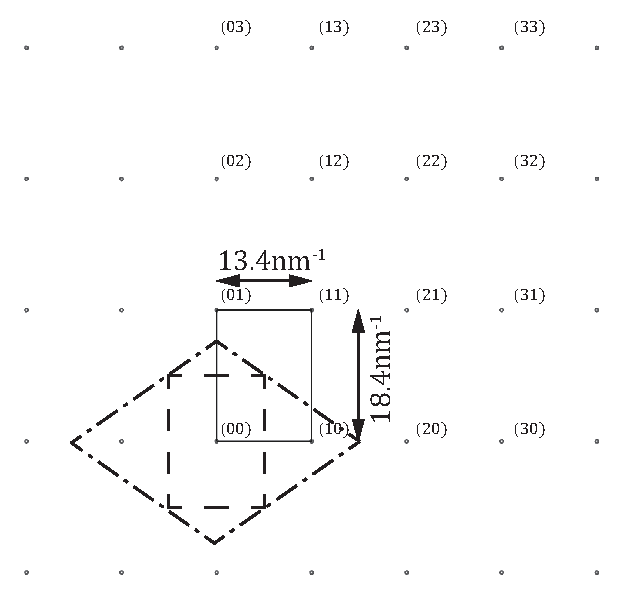
\includegraphics[width=.4\textwidth]{4.eps}
            \caption{二维正交晶格的倒格子.}
            \label{4-RL}
        \end{figure}
    \end{enumerate}
\end{sol}

\begin{prob}[(13.6) Brillouin Zones]
    \begin{enumerate}
        \item[(a)] Consider a cubic lattice with lattice constant $a$. Describe the first Brillouin zone. Given an arbitrary wavevector $\bm{k}$, write an expression for an equivalent wavevector within the first Brillouin zone (there are several possible expressions you can write).
        \item[(b)] Consider a triangle lattice in two dimensions (primitive lattice vectors given by Eqs. 12.3). Find the first Brillouin zone. Given an arbitrary wavevector $\bm{k}$ (in two dimensions), write an expression for an equivalent wavevector within the first Brillouin zone (again there are several possible expressions you can write).
    \end{enumerate}
\end{prob}
\begin{sol}
    \begin{enumerate}
        \item[(a)] 第一布里渊区为倒空间中$k_1,k_2,k_3\in[-\frac{\pi}{a},\frac{\pi}{a}]$范围内的区域. 对于任一个波矢$\bm{k}$,在第一布里渊区内的等价波矢为
        \begin{align}
            \bm{k}=\left[\begin{matrix}
                k_1-[[(k_1+\frac{\pi}{a})/(\frac{2\pi}{a})]]\times\frac{2\pi}{a}\\
                k_2-[[(k_1+\frac{\pi}{a})/(\frac{2\pi}{a})]]\times\frac{2\pi}{a}\\
                k_2-[[(k_1+\frac{\pi}{a})/(\frac{2\pi}{a})]]\times\frac{2\pi}{a}
            \end{matrix}\right]
        \end{align}
        其中$[[]]$为高斯符号,表示取不小于中括号内数的最大整数.
        \item[(b)] 该二维三角晶格的两个基矢为
        \begin{align*}
            \bm{a}_1=&a\hat{x},\\
            \bm{a}_2=&\frac{a}{2}\hat{x}+\frac{\sqrt{3}a}{2}\hat{y}.
        \end{align*}
        其倒格子的两个基矢分别为
        \begin{align*}
            \bm{b}_1=&\frac{2\pi\bm{a}_2\times\hat{z}}{\hat{z}\cdot(\bm{a}_1\times\bm{a}_2)}=\frac{2\pi}{a}(\hat{x}-\frac{\sqrt{3}}{3}\hat{y}),\\
            \bm{b}_2=&\frac{2\pi\hat{z}\times\bm{a}_1}{\hat{z}\cdot(\bm{a}_1\times\bm{a}_2)}=\frac{4\pi}{\sqrt{3}a}\hat{y}.
        \end{align*}
        如图\ref{5-RL},虚线所围区域即为第一布里渊区,是Weigner-Seitz形式的,当然布里渊区的选择不止一种,点划线所围区域是另一种第一布里渊区的形式.
        \begin{figure}[h]
            \centering
            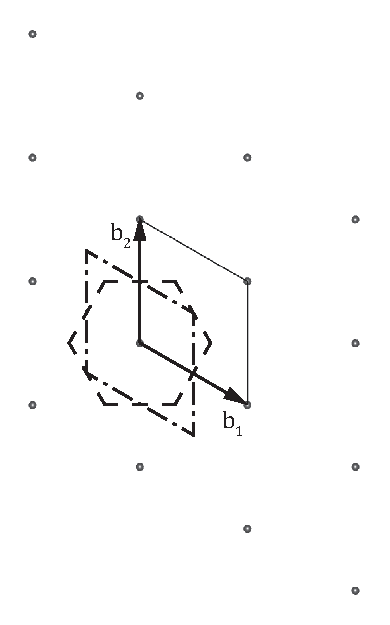
\includegraphics[width=.2\textwidth]{5.eps}
            \caption{二维三角晶格的倒格子.}
            \label{5-RL}
        \end{figure}
        \\任一个波矢$\bm{k}$可以写为倒格子的两个基矢的线性组合:
        \begin{align}
            \bm{k}=\alpha_1\bm{b}_1+\alpha_2\bm{b}_2.
        \end{align}
        由于
        \begin{align}
            \bm{k}\cdot\bm{b}_1=&\alpha_1\abs{\bm{b}_1}^2+\alpha_2\bm{b}_2\cdot\bm{b}_2=\frac{16\pi^2}{3a^2}\alpha_1-\frac{8\pi^2}{3a^2}\alpha_2,\\
            \bm{k}\cdot\bm{b}_2=&\alpha_2\bm{b}_1\cdot\bm{b}_2+\alpha_2\abs{\bm{b}_2}^2=-\frac{8\pi^2}{3a^2}\alpha_1+\frac{16\pi^2}{3a^2}\alpha_2.
        \end{align}
        故
        \begin{align}
            \alpha_1=&\frac{a^2}{8\pi^2}(2\bm{k}\cdot\bm{b}_1+\bm{k}\cdot\bm{b}_2),\\
            \alpha_2=&\frac{a^2}{8\pi^2}(\bm{k}\cdot\bm{b}_1+2\bm{k}\cdot\bm{b}_2).
        \end{align}
        与$\bm{k}$等价的第一布里渊区内的基矢为
        \begin{align}
            \bm{k}'=(\alpha_1-[[\alpha_1+\frac{1}{2}]])\bm{b}_1+(\alpha_2-[[\alpha_2+\frac{1}{2}]])\bm{b}_2.
        \end{align}
    \end{enumerate}
\end{sol}

\begin{prob}[(13.7) Number of States in the Brillouin Zone]
    A specimen in the form of a cube of side $L$ has primitive cubic lattice whose mutually orthogonal fundamental vectors (primitive lattice vectors) has length $a$. Show that the number of different allowed $\bm{k}$-states within the first Brillouin zone equals the number of primitive unit cells forming the specimen. (One may assume periodic boundary conditions, although it is worth thinking about whether whis still holds for hard-wall boundary conditions as well.)
\end{prob}
\begin{sol}
    在周期边界条件下,允许的$\bm{k}$的取值为
    \begin{align*}
        \bm{k}=[h,k,l]\frac{2\pi}{L}.
    \end{align*}
    可见每个$k$平均对应着倒空间中$\left(\frac{2\pi}{L}\right)^3$的体积. 而第一布里渊区为倒空间中$k_1,k_2,k_3\in[-\frac{\pi}{a},\frac{\pi}{a}]$范围内的区域. 故在第一布里渊区中的倒格点数量为
    \begin{align*}
        \frac{\left(2\frac{\pi}{a}\right)^3}{\left(\frac{2\pi}{L}\right)^3}=\frac{L^3}{a^3}.
    \end{align*}
    该样品中的原胞数量为样品总体积和原胞体积之商:
    \begin{align*}
        \frac{L^3}{a^3}.
    \end{align*}
    因此第一布里渊区内允许的$\bm{k}$的数量与样品中的原胞数量相等.
\end{sol}
\end{document}